\section{Results}
    \subsection{Positioning}
    \begin{frame}{Results: Positioning}
            \centering
            \begin{minipage}{\linewidth}
                \centering
                \includegraphics[trim = 0mm 50mm 0mm 0mm,clip,width=0.5\textwidth]{\currentchapter/figures/X}
                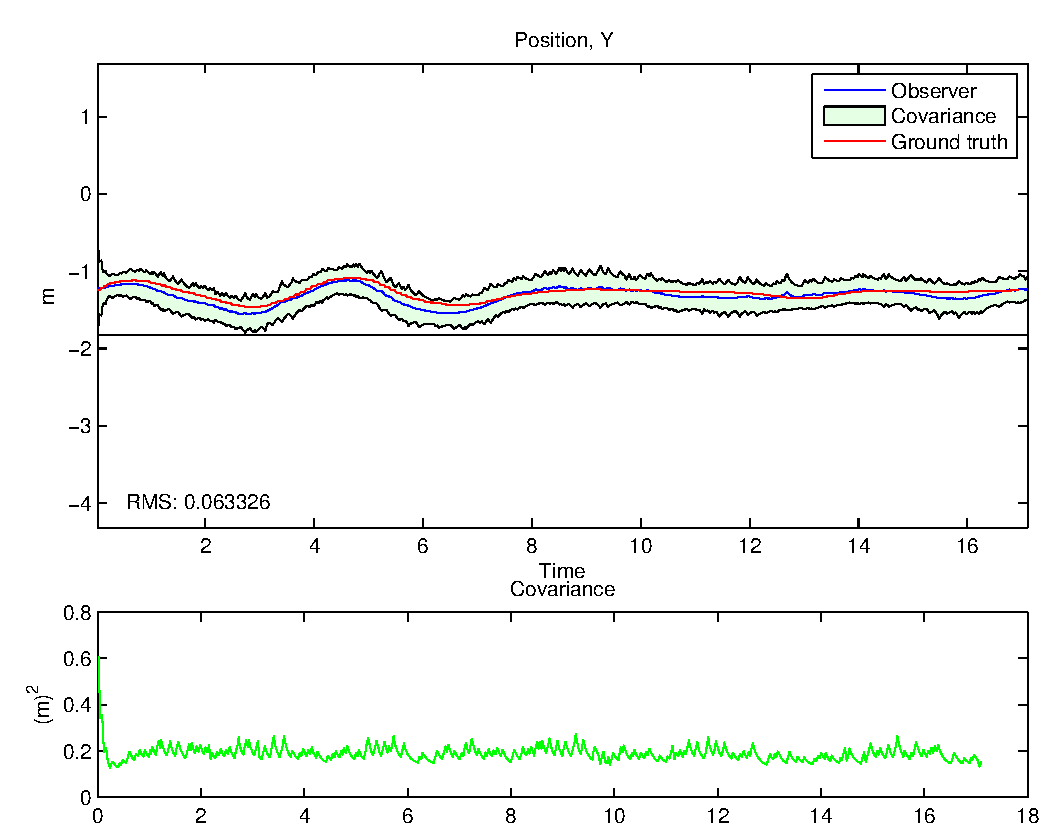
\includegraphics[trim = 0mm 50mm 0mm 0mm,clip,width=0.5\textwidth]{\currentchapter/figures/Y}\\
                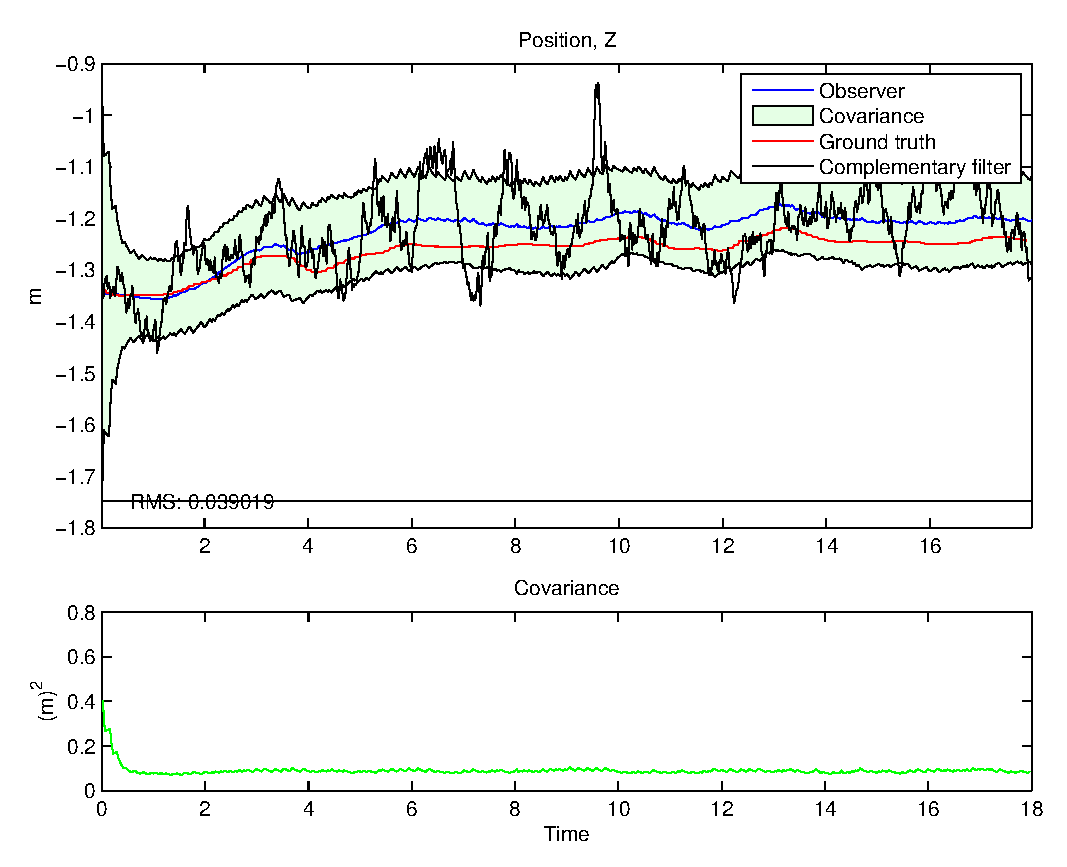
\includegraphics[trim = 0mm 50mm 0mm 0mm,clip,width=0.8\textwidth]{\currentchapter/figures/Z}
            \end{minipage}
    \end{frame}
    \note{
        I will now present a very brief excerpt from the results that were
        obtained.

        As a result of connecting the camera localization to the quadrotor positioning,
        the fused measurements yield high precision.
        For the altitude, the complementary filter is shown in comparison.

        We can see that the camera positioning contribute with stable
        positioning and precision, while the complementary filter suffers
        from its dependency on the noisy pressure sensor, which is very difficult to
        use indoors.
    }

    \subsection{Control}
    \begin{frame}{Results: Control}
        \fig{0.9}{referencefollowing}
    \end{frame}
    \note{
        With precision state estimation, the quadrotor was put through a
        simulated testflight. This testflight displays the proposed controller's
        ability to follow a reference trajectory and land the LinkQuad.

        The flight started of with a sinusoid reference.
        The state-machine then enters the landing procedure and halts the vehicle
        before starting its descent.
    }
